\chapter{Modellierung}
In diesem Kapitel sollen die Anforderungen aus den Interviews praktisch erhoben werden, die Referenzarchitekturen erstellt werden und die konstruierten Referenzarchitekturen folgend auch verglichen werden.
\section{Anforderungserhebung}
Wie in \autoref{theorie:referenzmodellierung} beschrieben, müssen Referenzmodelle einen subjektiven Empfehlungscharakter besitzen, damit sie akzeptiert und wiederverwendet werden. Dafür muss ein Abgleich mit den Anforderungen der Nutzenden geschehen. Um dies zu erreichen, wurden im Anhang transkribierte Interviews (vgl. Anhang~\ref{chap:interview-philipp-22.03.2021},\ref{chap:interview-peter-24.03.2021},\ref{chap:interview-ralph-24.03.2021}) durchgeführt. Daraus ergibt sich das in \autoref{abb:TopLevelEchtzeitRA} gezeigte Diagramm, welches die Anforderungen der individuellen Stakeholder an Dekompositiontiefe, Anwendbarkeit und Allgemeingültigkeit darstellt.

\begin{figure}[H]
\centering
\spideroverview
%{P. Arnold}
{5}{3}{3}
%{R. Briegel}
{3}{3}{1}
%{P. Erbacher}
{2}{4}{5}
\caption{Ergebnisse der Interviews}
\label{abb:DimensionenUebersicht}
\end{figure}
Durch die Interviews liessen sich folgende Durchschnitte errechnen: Dekompositionstiefe wurde im Schnitt mit $3,\overline{3}$ bewertet. Die Anwendbarkeit wurde ebenfalls mit $3,\overline{3}$ bewertet. Die Allgemeingültigkeit hingegen hat nur einen Schnitt von $3$/5. Entsprechend sollten Dekompositionstiefe und Anwendbarkeit priorisiert werden.

Zusätzlich haben sich folgende Anforderungen ergeben:
\begin{itemize}
\item Anwendbarkeit auf Monitoring (klassische IT)
\item Anwendbarkeit auf Sensordaten (\ac{IoT})
\item Wertschöpfung für den Betrieb wichtig
\item akzeptabel und problemlösend für Domäne
\item Handling von Events, Messwerten und \enquote{Streaming}
\end{itemize}

\section{Echtzeitverarbeitung}
\subsection{Ablauf}
\begin{figure}[H]
\centering
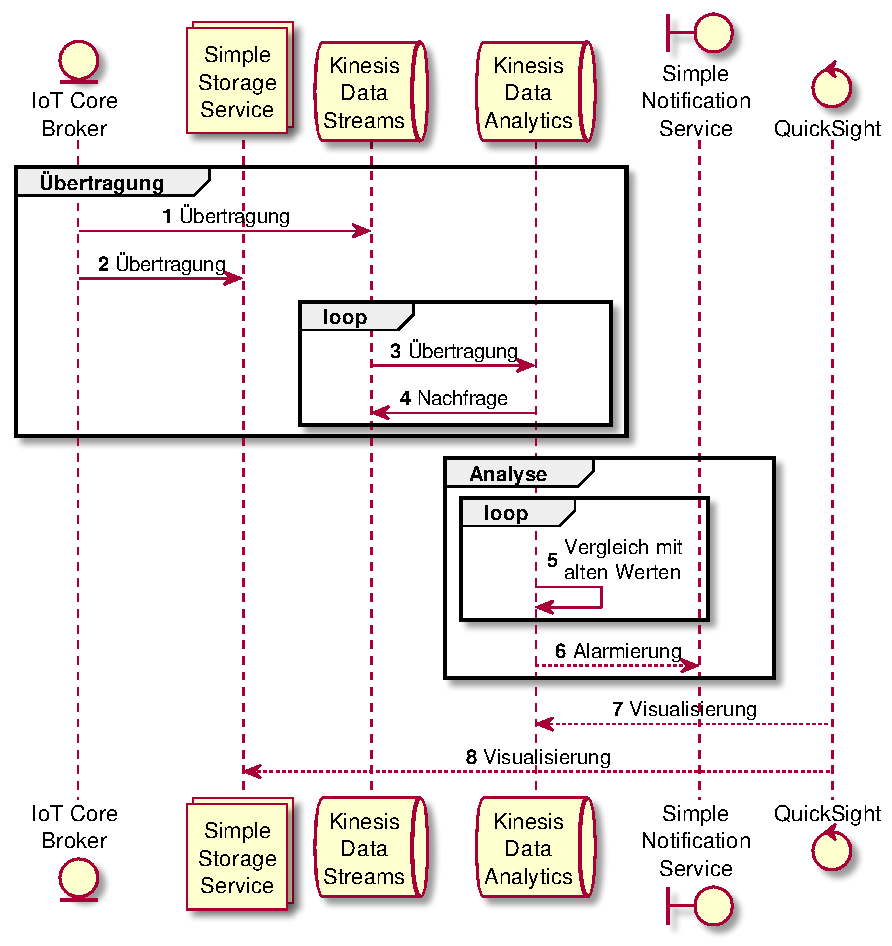
\includegraphics[width=\textwidth]{graphics/echtzeit-ra.pdf}
\caption{Sequenzdiagramm}
\label{abb:SequenceEchtzeitRA}
\end{figure}

\subsection{Interagierende Elemente}
\begin{figure}[H]
\centering
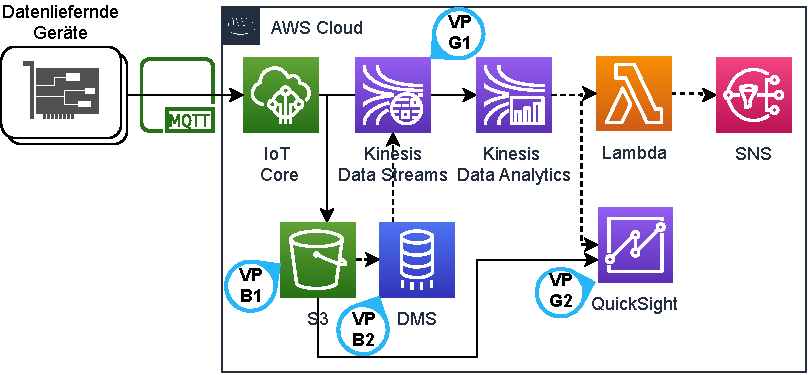
\includegraphics[width=\textwidth]{graphics/Echtzeit-RA-Overview.pdf}
\caption{Top Level View Referenzarchitektur}
\label{abb:TopLevelEchtzeitRA}
\end{figure}
Variationspunkt 1: Rohdaten in \ac{S3} zu speichern kann Sinn machen, um die Daten später noch einmal analysieren zu können. Nimmt man aber die Theorie der Datenhalbwertszeit zur Hilfe, macht es vielleicht Sinn die Daten statdessen maximal 48h in Kinesis zwischenzuspeichern und auf \ac{S3} zu verzichten.

Variationspunkt 2: \ac{DMS} ist in diesem Szenario dafür gedacht, einmal abgelegte Daten in S3 wieder in Kinesis Data Streams einspielen zu können. Je nach Szenario macht das, wie bei Variationspunkt 1 schon erläutert, wenig Sinn.

Variationspunkt 3: QuickSight als \ac{AWS} native Dashboardlösung ist gut geeignet, um schnell Übersicht in Datenanalysen aus Kinesis Data Analytics zu bekommen. Alternativ können auch andere Visualisierungslösungen wie Tableau eingesetzt werden, welche gegebenenfalls jedoch nicht auf Kinesis Data Analytics zugreifen können. In solch einem Fall kann es Sinn machen, den aus Variationspunkt 1 bekannten \ac{S3} Bucket aufzusetzen, um Dashboards über die Rohdaten erstellen zu können.

\subsection{Interagierende Elemente - Ebene 2}
\begin{figure}[H]
\centering
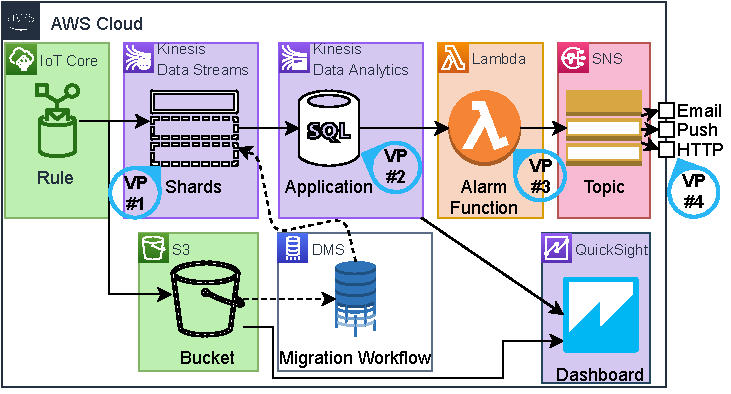
\includegraphics[height=0.33\textheight]{graphics/Echtzeit-RA-Elements.pdf}
\caption{Interagierende Dienstelemente}
\label{abb:ElementeEchtzeitRA}
\end{figure}
Variationspunkt 1: Die Anzahl an Shards ist esentiell für die Performance von Kinesis Data Streams. Für Workloads mit einem vorhersehbaren Workload ist eine Preis/Leistungs optimale Anzahl an Shards zu ermitteln und zu konfigurieren. Wenn der Workload nicht vorhersehbar ist oder schnell skalieren können soll, sind Alarme im AWS eigenen Monitoring Tool CloudWatch zu erstellen. Im Beispielusecase für die Kostenschätzung wäre beispielsweise ein einziger Shard (1MiB/Sekunde, 1000 Nachrichten eingehend) ausreichend, da Nachrichten mit einer Größe von 1KB, also \~1KiB geschrieben werden, bei einem Maximum von 200 pro Sekunde und einem Konsumenten. Es ist besonders auf die \enquote{WriteProvisionedThroughputExceeded} Metrik zu achten, welche bei höheren Werten anzeigt, dass das Hinzufügen von zusätzlichen Shards angebracht wäre. Ebenfalls ist die Metrik \enquote{Incoming Records} zu beachten. Verändert diese sich, deutet das auf einen Fehler im vorgelagerten \AWSIOT Core oder in einem Teil der Datenlieferanten hin.

Variationspunkt 2: Der \ac{SQL} Programmcode, der in Kinesis Data Analytics läuft ist anzupassen. So sind Verarbeitungsfenster, Attributsnamen und aufgerufene Funktionen nach Anforderung zu ändern. Andernfalls kann auch die Funktionalität zur Ausführung eigenen Codes via Apache Flink in Kinesis Data Analytics genutzt werden (dies erlaubt Ausführung von Java, Scala, Python).


\section{Batch Verarbeitung}



\begin{figure}[H]
\centering
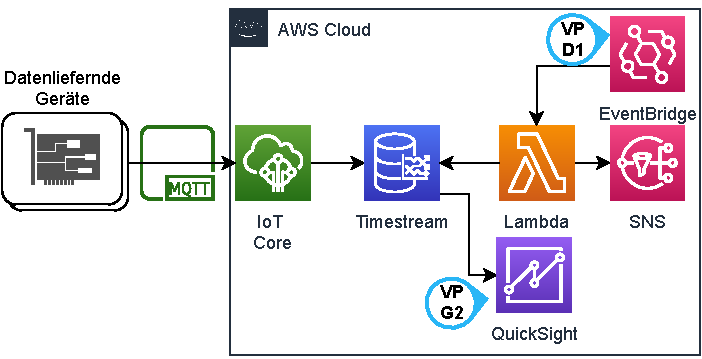
\includegraphics[width=\textwidth]{graphics/DB-RA-Overview.pdf}
\caption{Top Level View Referenzarchitektur}
\label{abb:TopLevelDBRA}
\end{figure}



\begin{figure}[H]
\centering
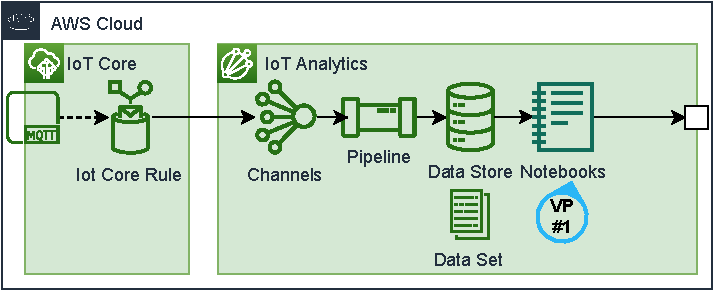
\includegraphics[width=\textwidth]{graphics/DB-RA-Elements.pdf}
\caption{Interagierende Dienstelemente}
\label{abb:ElementeDBRA}
\end{figure}

\section{Einsatzszenarien der Referenzmodelle}


Chaos Engineering nicht vergessen \footcite[Vgl.][]{Augsten.2020}

Innerhalb dieser Arbeit wurden Referenzarchitekturen für die Verarbeitung in der Cloud konstruiert. Ein Trend, der dabei ausgespart wurde, ist das sogenannte \enquote{Fog computing}. Nach der Definition von \citeauthor{Vaquero.2014} ist Fog computing ein Szenario, in dem heterogene, allgegenwärtige und dezentralisierte Geräte kommunizieren und kooperieren um Speicher- und Verarbeitungsaufgaben zu übernehmen.\footcite[Vgl.][30\psq]{Vaquero.2014} In der Praxis führt dies dazu, dass Verarbeitungsaufgaben in Teilen, angelehnt an das \enquote{Edge computing} von der Cloud in Richtung der Geräte ausgelagert wird.\footcite[Vgl.][]{Bonomi.2012} Dies geschieht dabei beispielsweise an Netzwerkgateways, die sowieso mit der Cloud kommunizieren und folgend nur noch bereits ausgewertete Daten übertragen.